\documentclass[twocolumn,preprintnumbers,superscriptaddress]{revtex4-2}
\usepackage{amsmath}
\usepackage{amssymb}
\usepackage{graphicx}
\usepackage{hyperref}
\usepackage{physics}
\usepackage{xcolor}
\usepackage{xspace,slashed}
\usepackage{qcircuit}
\usepackage{multirow}
\usepackage[utf8]{inputenc}
\usepackage{subfigure}

\usepackage{array}

\begin{document}

\title{
  Generating LHC events with a quantum generative model
 }

\preprint{CERN-TH-xx, TIF-UNIMI-2021-xx}

\newcommand{\CERNaff}{Theoretical Physics Department, CERN, CH-1211
  Geneva 23, Switzerland.}

\newcommand{\tii}{Quantum Research Centre, Technology Innovation Institute, Abu Dhabi, UAE}

\newcommand{\bern}{Albert Einstein Center, CH-3012 Bern, Switzerland}

\newcommand{\UB}{Departament de F\'isica Qu\`antica i Astrof\'isica and Institut de Ci\`encies del Cosmos (ICCUB), Universitat de Barcelona, Barcelona, Spain.}

\newcommand{\MIaff}{TIF Lab, Dipartimento di Fisica, Universit\`a degli Studi di
  Milano and INFN Sezione di Milano, Milan, Italy.}

\author{Carlos Bravo-Prieto}
\affiliation{\tii}
\affiliation{\UB}

\author{Julien Baglio}
\affiliation{\CERNaff}

\author{Marco C\`e}
\affiliation{\CERNaff}

\author{Anthony Francis}
\affiliation{\bern}

\author{Dorota Grabowska}
\affiliation{\CERNaff}

\author{Stefano Carrazza}
\affiliation{\MIaff}
\affiliation{\CERNaff}
\affiliation{\tii}


\begin{abstract}
    We present a first attempt to design a quantum circuit for the generation of
    Monte Carlo simulated events using quantum generative models, in the context
    of high energy physics (HEP). The growing interest in quantum computing and
    the recent developments of new algorithms and quantum hardware devices
    motivates the study of methodologies applied to HEP. In this work we
    identify architectures of variational quantum circuits suitable for
    designing a generative model for Monte Carlo event generation. We validate
    the methodology by performing experiments on artificial data generated from
    known underlying distributions. Finally, we model Monte Carlo simulated
    events and benchmark the performance in terms of quality and performance.
\end{abstract}

\maketitle

\section{Introduction}
Quantum computing is a new paradigm whereby quantum phenomena are harnessed to perform computations. The current availability of noisy intermediate-scale quantum computers (NISQ)~\cite{nisq}, and recent achievements such as quantum computational supremacy~\cite{supremacy, zhong2020quantum}, have led to a growing interest in these devices to perform computational tasks faster than any classical machine. Among many of the near-term applications~\cite{cerezo2021variational, bharti2021noisy}, the field of Quantum Machine Learning (QML)~\cite{biamonte2017quantum, schuld2018supervised} is held as one of the most promising approaches to make use of NISQ computers.

Early work in QML was mostly focused on speeding up linear algebra subroutines~\cite{wiebe2012quantum, lloyd:2013ml, Rebentrost:2014svm, kerenidis2020quantum}, widely used in classical machine learning, by leveraging the HHL algorithm~\cite{harrow2009quantum}. Notice that this approach holds promise for the future, when large-scale quantum computers exist with low gates errors and enough qubits for quantum error correction. On the other hand, more recent proposals suggest using the quantum devices to define a parameterized quantum circuit~\cite{benedetti2019parameterized, sim2019expressibility, bravo2020scaling}, or quantum neural network (QNN), which then can be trained to implement a function class~\cite{schuld2021effect, goto2021universal, perez2021one}. For example, several QNNs have been proposed for pattern classification~\cite{havlivcek2019supervised, Schuld:2020circuit, perezsalinas:2020reuploading} or data compression~\cite{romero2017quantum, bravo2021quantum, cao2021noise}. Interestingly, this QML approach to quantum computing is a research topic that can be adapted, improved, and tested on many research problems. Motivated by this idea, we propose to investigate the possibility to use QNNs for generative modeling~\cite{benedetti2019generative, hamilton2019generative, coyle2020born}. More specifically, for the generation of Monte Carlo events through quantum generative adversarial networks (qGANs)~\cite{dallaire2018quantum, lloyd2018quantum}.

The generative adversarial framework employs two competing networks that are trained alternatively, the generator and the discriminator~\cite{goodfellow2014generative}. The generator produces candidates while the discriminator evaluates them. The objective of the discriminator is to distinguish the real samples from the generated ones. That is, the discriminator plays the role of the generator's adversary, and therefore, their competition is a zero-sum two-player game. Substituting either the discriminator, the generator, or both with quantum systems we translate the scheme to quantum computing.

In recent months, the spreading interest in QML has led to different qGAN implementations~\cite{zoufal2019quantum, zeng2019learning, situ2020quantum, hu2019quantum, benedetti2019adversarial, romero2021variational, niu2021entangling}. However, our contribution here can be summarized in three distinct aspects. (1) Previous proposals employ toy data for their qGAN training. Moreover, in some cases, it is classical data. It has been recently conjectured that if QML ever provides any speed up, it will likely appear from learning the data of a quantum process~\cite{huang2021information, kubler2021inductive}. We, therefore, train our qGAN model with artificial LHC data. (2) We propose an alternative quantum generator architecture. In contrast to previous proposals where the prior noise distribution, or latent dimension, is encoded at the beginning of the generator, we instead encode it on every layer of the network. This permits to the new generator to process and decide in which parts of the network the latent variables should play a relevant role. This allowed us to achieve improved state-of-the-art results with shallow QNNs using adversarial learning. Let us remark as well that this has been proven extremely useful in the classical context~\cite{karras2019style}. (3) We validate and assess our qGAN in quantum hardware. Specifically, we successfully implement our model in two different quantum architectures, namely, ion traps and superconducting qubits.

% To be modified
The paper is structured as follows. Sec.~\ref{sec:implementation} we identify
the best {\tt QGMC} architecture. In Sec.~\ref{sec:validation} we validate the
{\tt QGMC} model using toy data. In Sec.~\ref{sec:lhc} we train the {\tt QGMC}
generator on simulated LHC events. Finally, in Sec.~\ref{sec:deployment} we test
our final model on real quantum hardware and in Sec.~\ref{sec:conclusion} we
present our conclusion and future development directions.

\section{Implementation}
\label{sec:implementation}

\begin{enumerate}
  \item Talk about model definition
  \item Talk about training procedure
\end{enumerate}

\begin{figure*}
  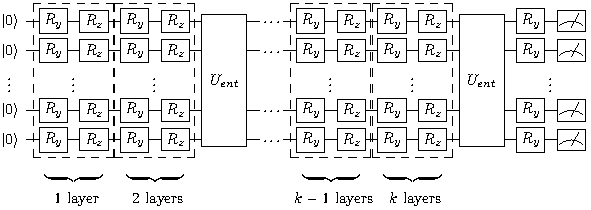
\includegraphics[width=0.8\textwidth]{plots/ansatz1.pdf}
  \caption{\label{fig:circuit}Ansatz 1 for the quantum generator.}
\end{figure*}

\section{Validation}
\label{sec:validation}

\begin{enumerate}
  \item Show 1D example (histograms + KL) for different (layers, latent) dim.
  \item Show 2D example (histograms + KL) for different (layers, latent) dim.
  \item Show 3D gaussian example for different (layers, latent) dim.
\end{enumerate}

\begin{figure}
  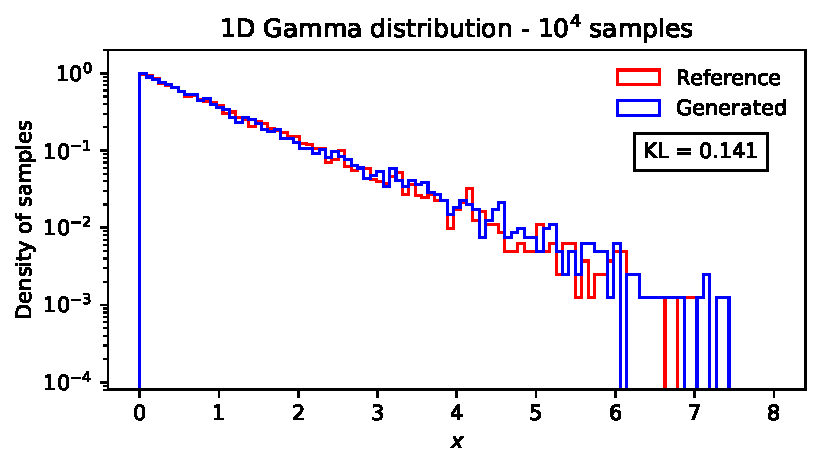
\includegraphics[width=0.45\textwidth]{plots/1Dgamma/1Dgamma_distribution_10k.pdf}
  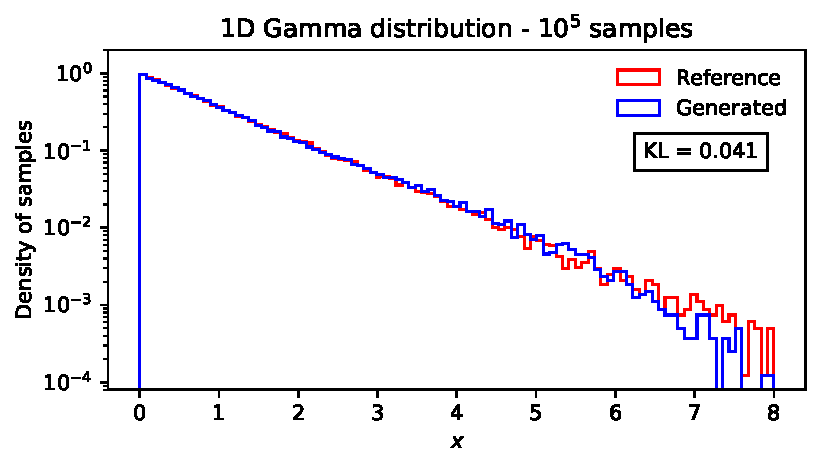
\includegraphics[width=0.45\textwidth]{plots/1Dgamma/1Dgamma_distribution_100k.pdf}
  \caption{Example of 1D gamma distribution.}
\end{figure}


\begin{figure}
  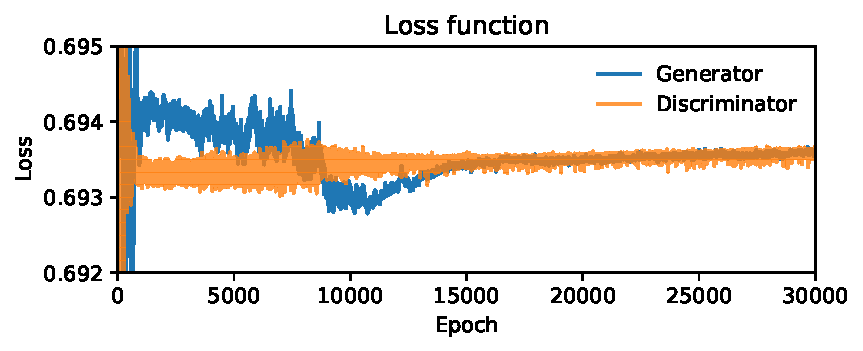
\includegraphics[width=0.5\textwidth]{plots/1Dgamma/1Dgamma_loss.pdf}
  \caption{Example of 1D gamma distribution.}
\end{figure}

\begin{figure*}
  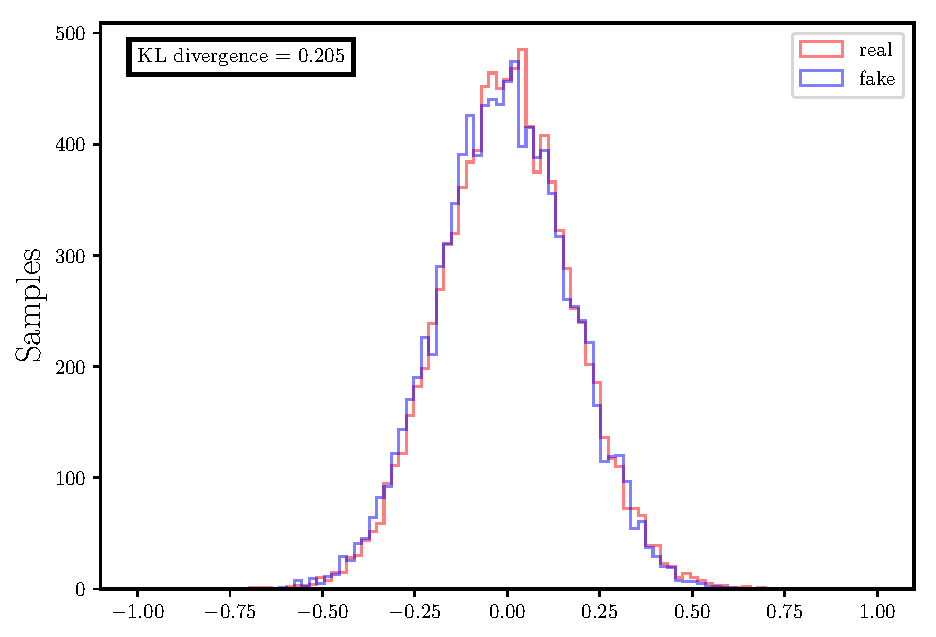
\includegraphics[width=0.25\textwidth]{plots/3Dgaussian_posdef/1-distribution_10000_100_3_5_2_10000_128_0.5.pdf}%
  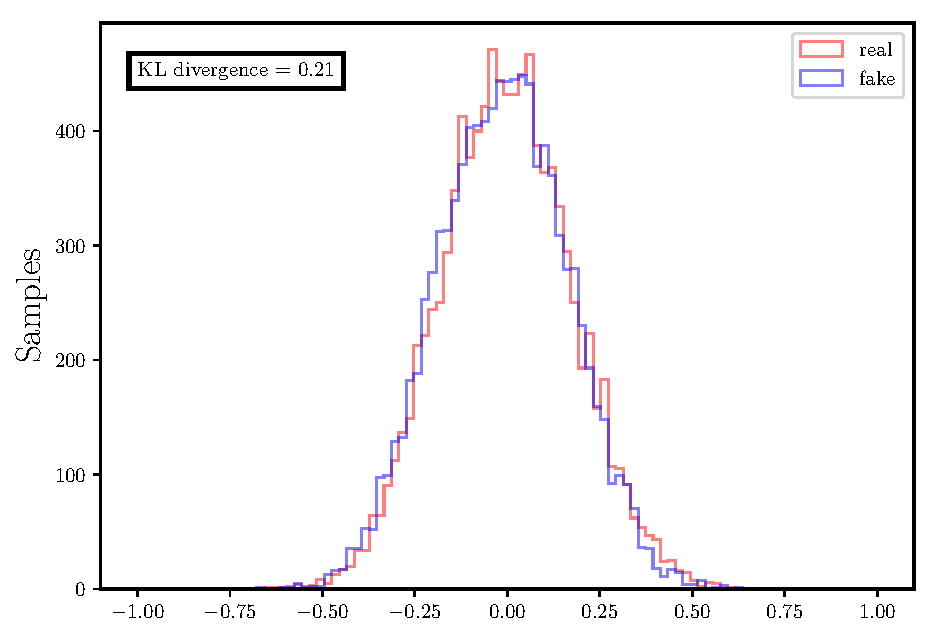
\includegraphics[width=0.25\textwidth]{plots/3Dgaussian_posdef/2-distribution_10000_100_3_5_2_10000_128_0.5.pdf}%
  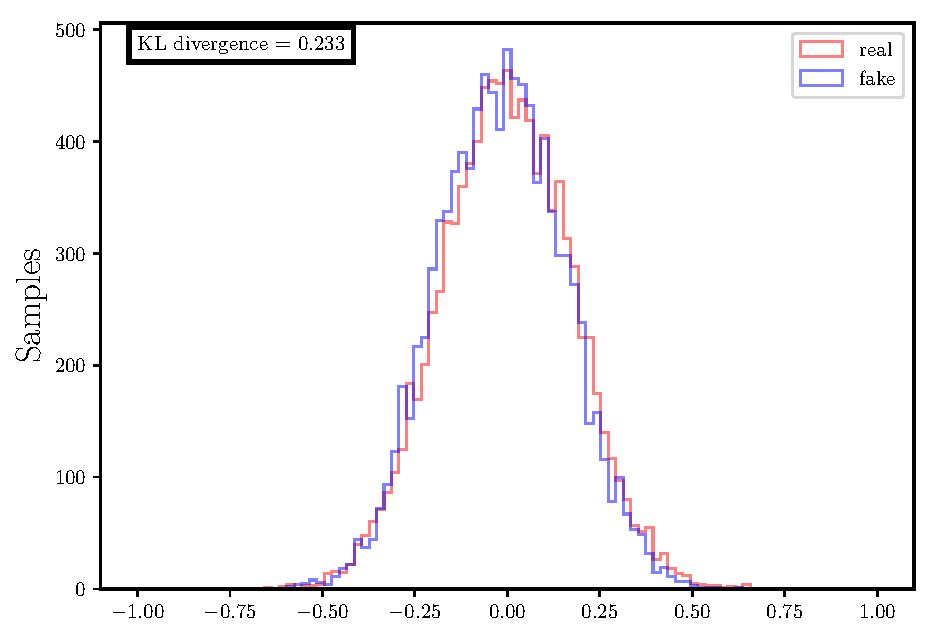
\includegraphics[width=0.25\textwidth]{plots/3Dgaussian_posdef/3-distribution_10000_100_3_5_2_10000_128_0.5.pdf}

  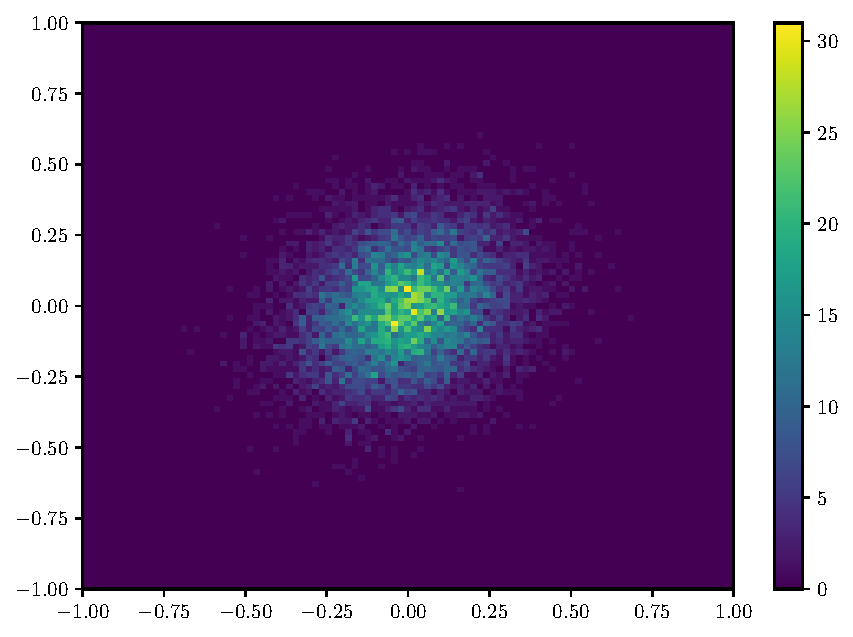
\includegraphics[width=0.25\textwidth]{plots/3Dgaussian_posdef/1-2_REAL_10000_100.pdf}%
  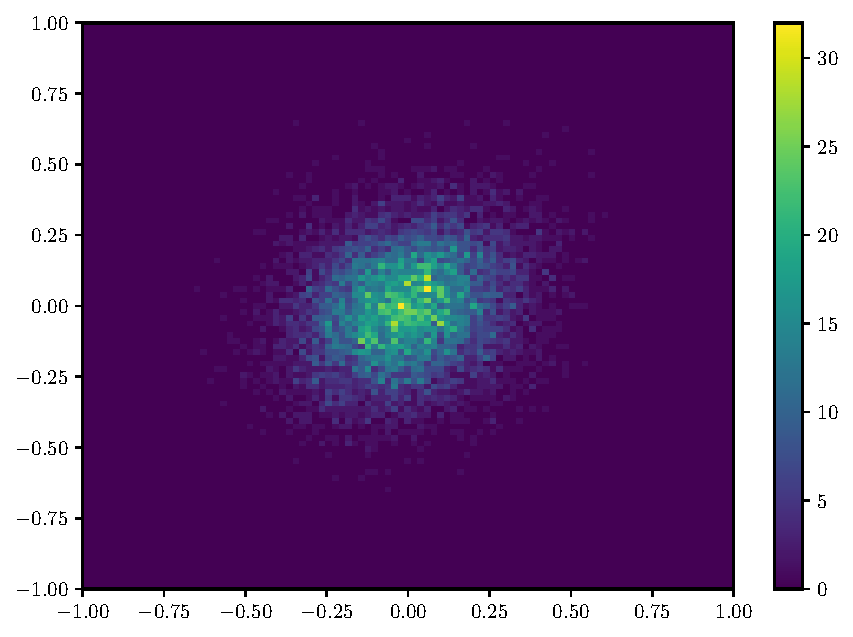
\includegraphics[width=0.25\textwidth]{plots/3Dgaussian_posdef/2-3_REAL_10000_100.pdf}%
  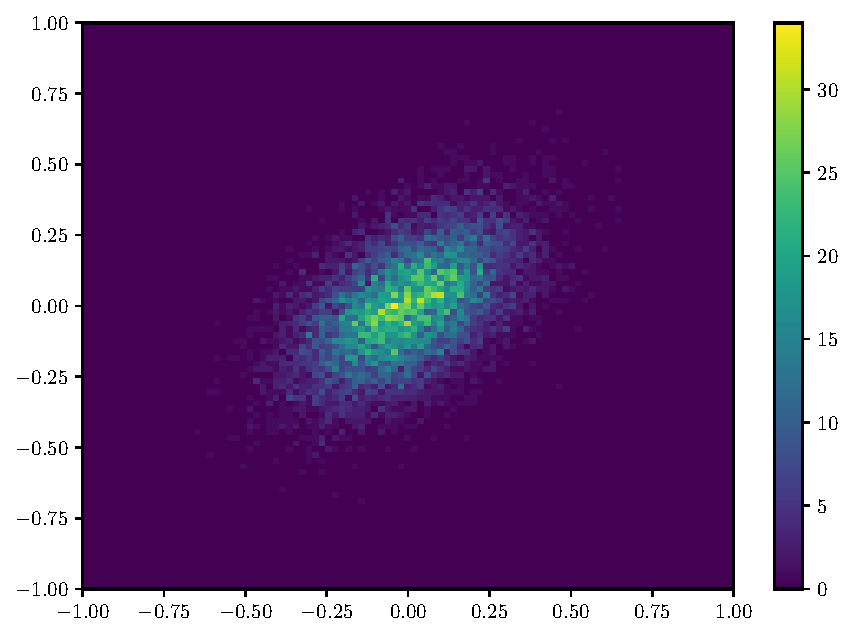
\includegraphics[width=0.25\textwidth]{plots/3Dgaussian_posdef/3-1_REAL_10000_100.pdf}

  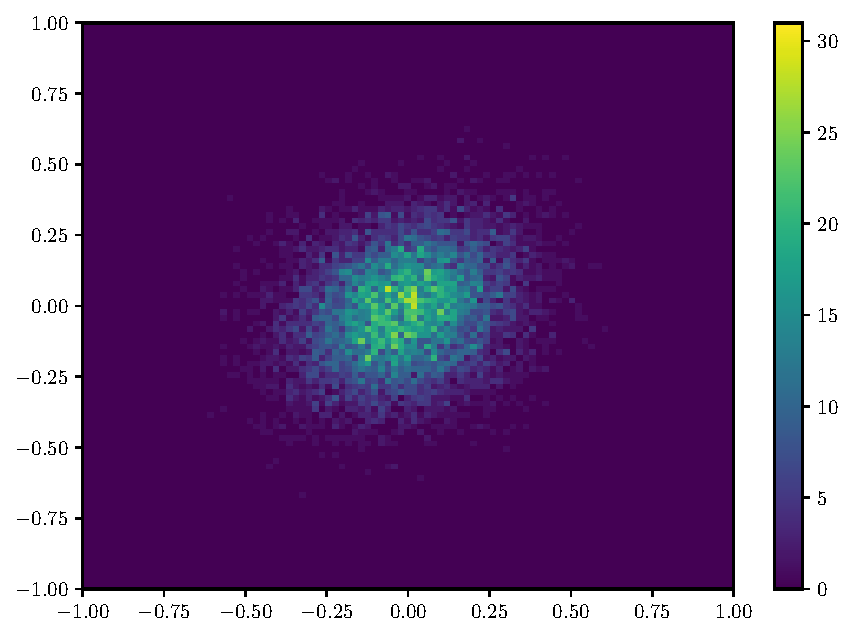
\includegraphics[width=0.25\textwidth]{plots/3Dgaussian_posdef/1-2_FAKE_10000_100_3_5_2_10000_128_0.5.pdf}%
  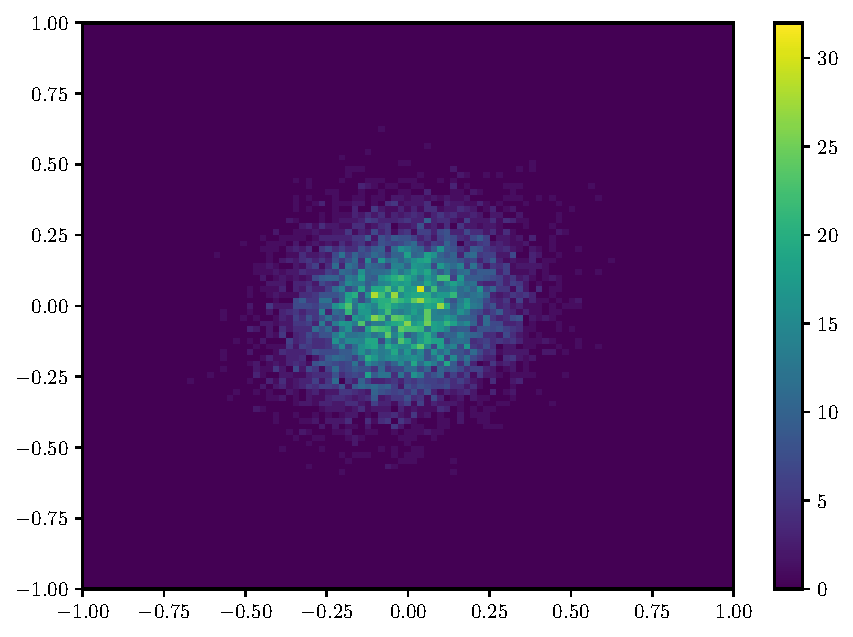
\includegraphics[width=0.25\textwidth]{plots/3Dgaussian_posdef/2-3_FAKE_10000_100_3_5_2_10000_128_0.5.pdf}%
  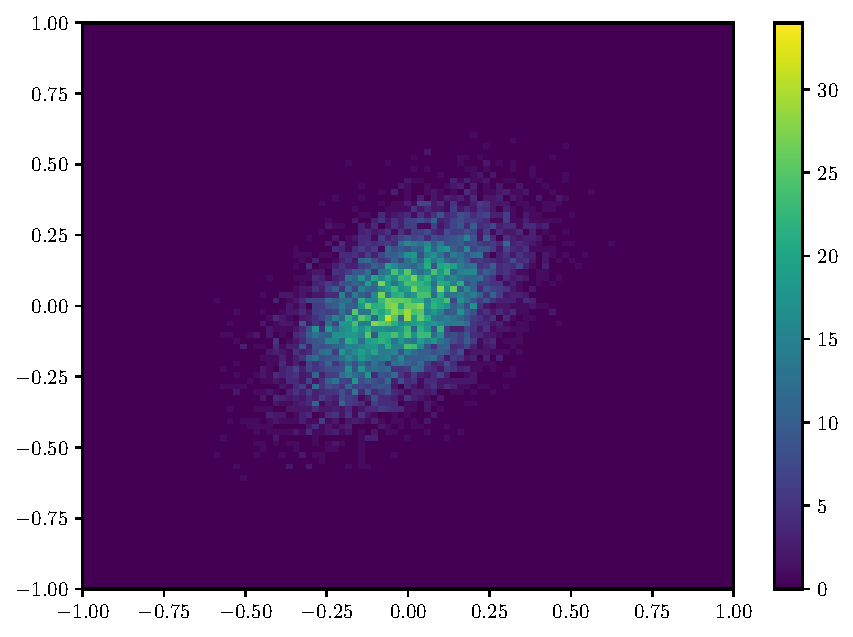
\includegraphics[width=0.25\textwidth]{plots/3Dgaussian_posdef/3-1_FAKE_10000_100_3_5_2_10000_128_0.5.pdf}
  \caption{\label{fig:3dgauss}Example of samples generated for a 3D correlated
  multivariate normal distribution using a QGAN generator model.}
\end{figure*}

\begin{figure*}
  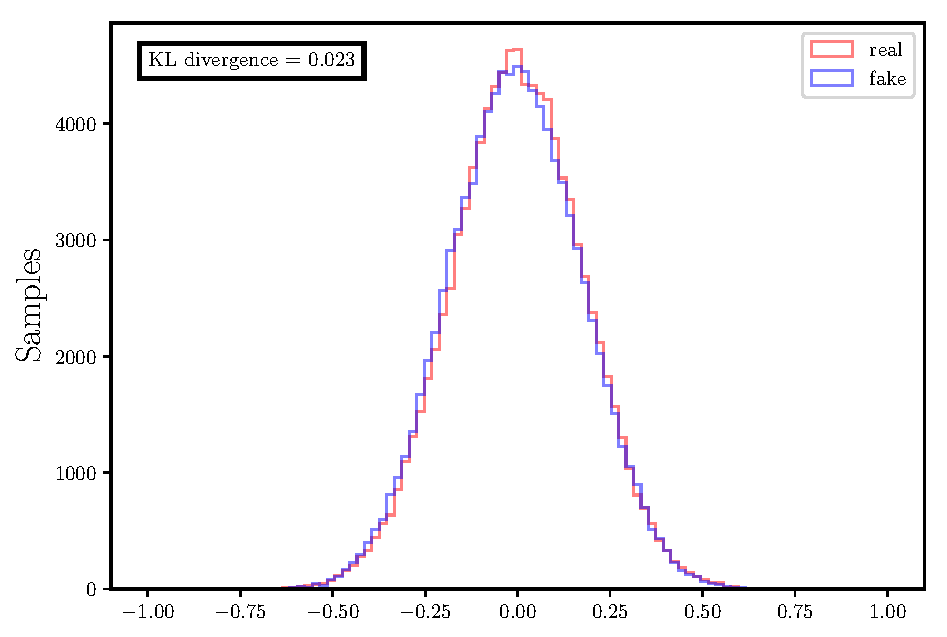
\includegraphics[width=0.25\textwidth]{plots/3Dgaussian_posdef/1-distribution_100000_100_3_5_2_10000_128_0.5.pdf}%
  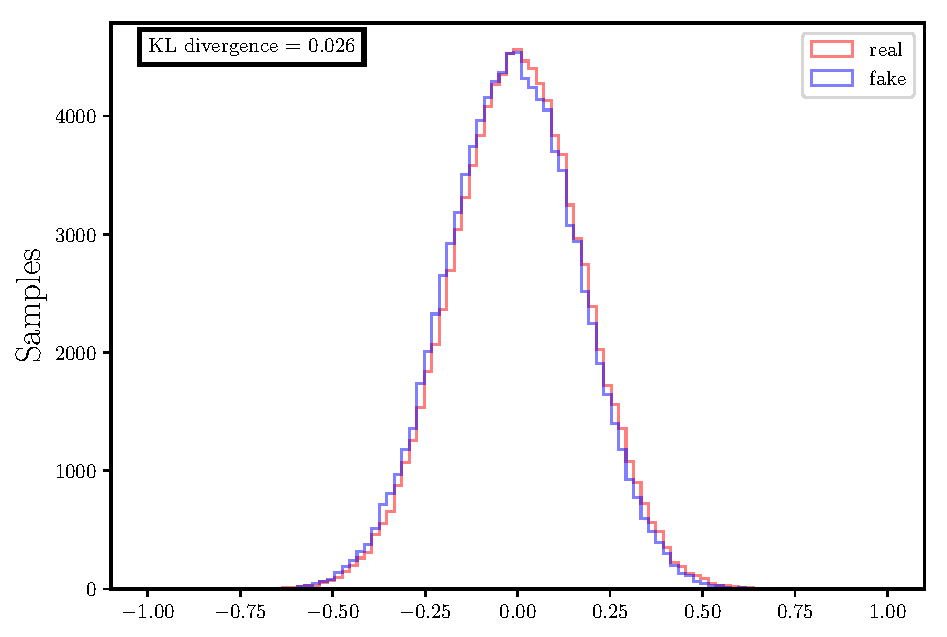
\includegraphics[width=0.25\textwidth]{plots/3Dgaussian_posdef/2-distribution_100000_100_3_5_2_10000_128_0.5.pdf}%
  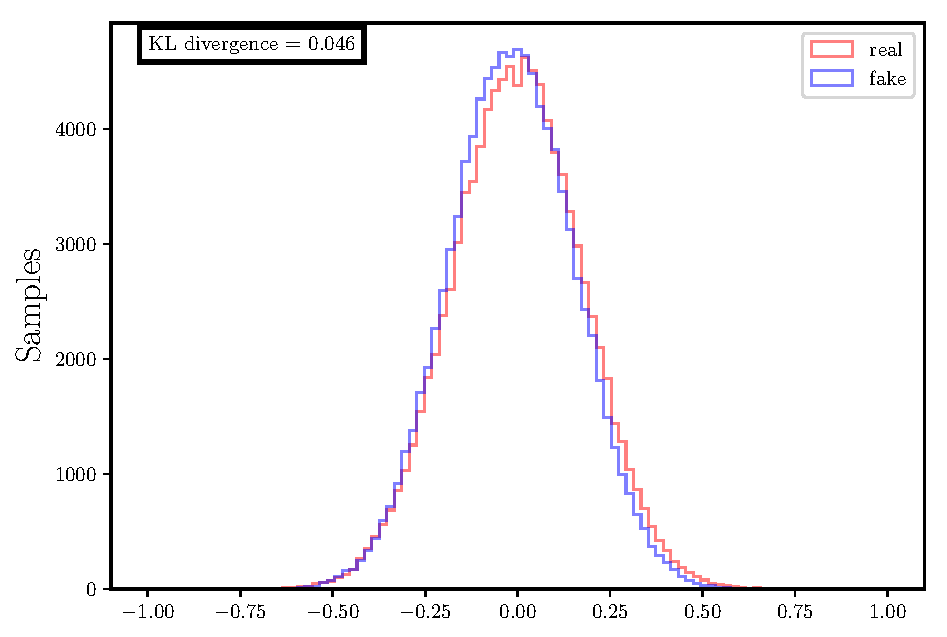
\includegraphics[width=0.25\textwidth]{plots/3Dgaussian_posdef/3-distribution_100000_100_3_5_2_10000_128_0.5.pdf}

  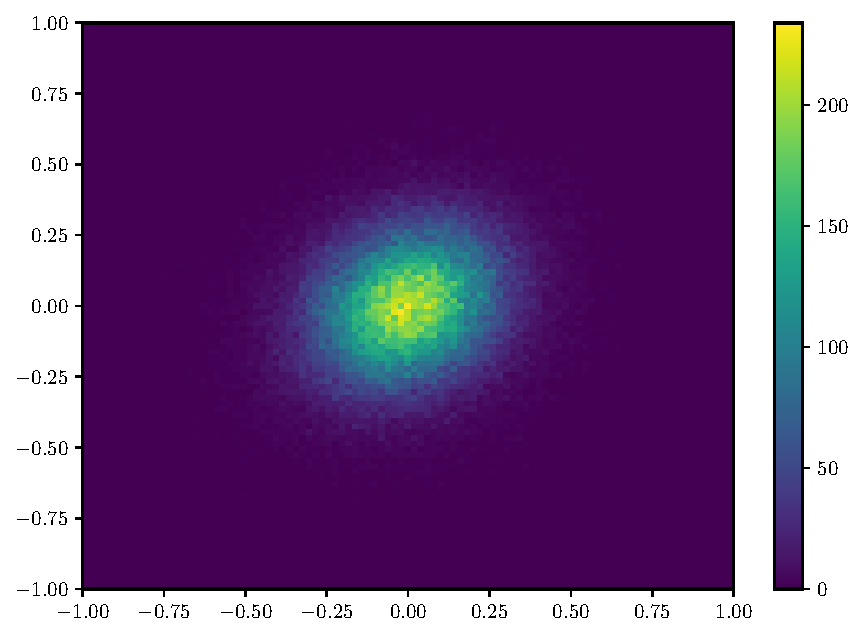
\includegraphics[width=0.25\textwidth]{plots/3Dgaussian_posdef/1-2_REAL_100000_100.pdf}%
  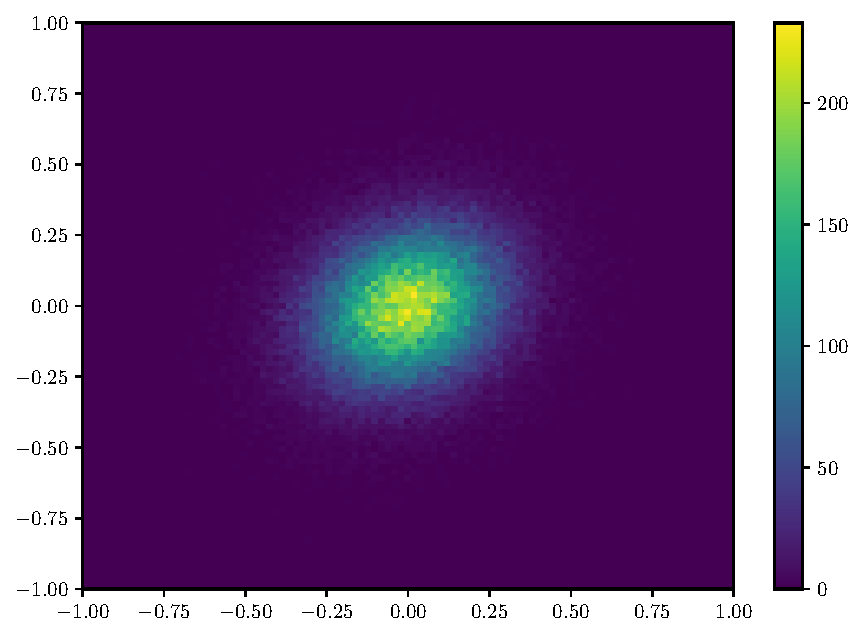
\includegraphics[width=0.25\textwidth]{plots/3Dgaussian_posdef/2-3_REAL_100000_100.pdf}%
  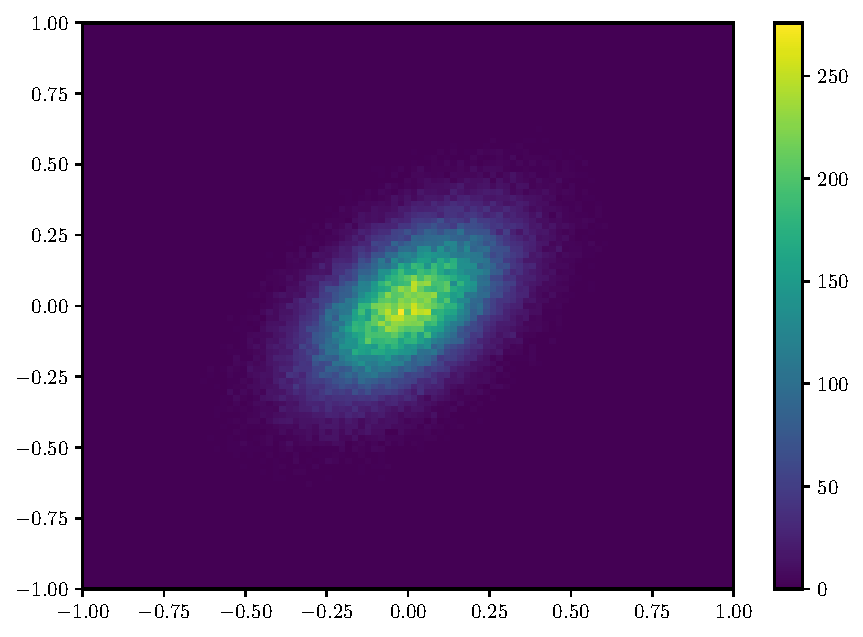
\includegraphics[width=0.25\textwidth]{plots/3Dgaussian_posdef/3-1_REAL_100000_100.pdf}

  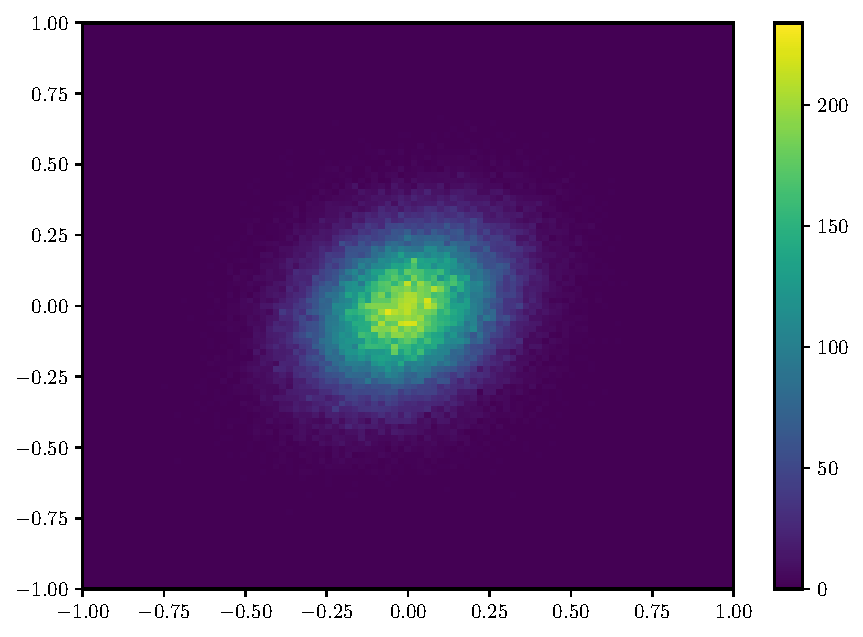
\includegraphics[width=0.25\textwidth]{plots/3Dgaussian_posdef/1-2_FAKE_100000_100_3_5_2_10000_128_0.5.pdf}%
  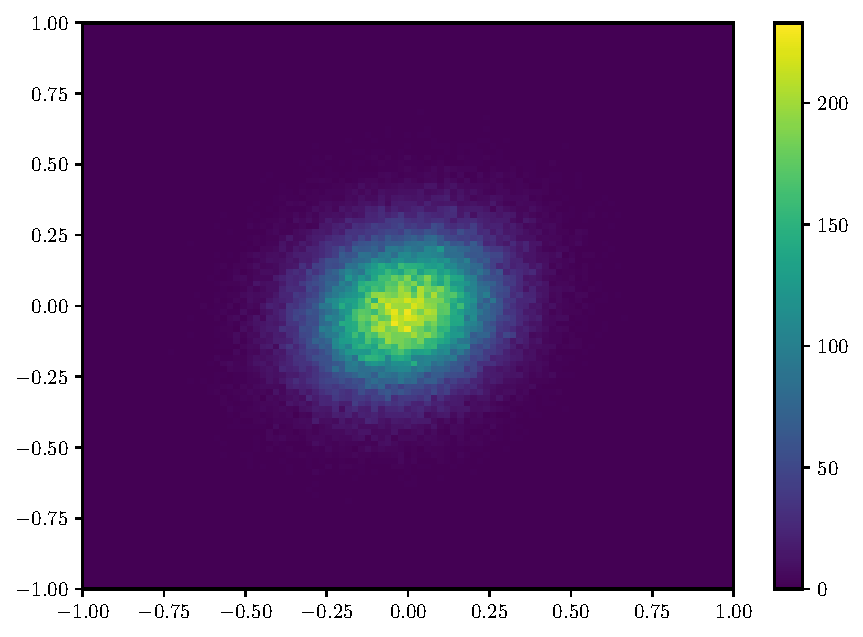
\includegraphics[width=0.25\textwidth]{plots/3Dgaussian_posdef/2-3_FAKE_100000_100_3_5_2_10000_128_0.5.pdf}%
  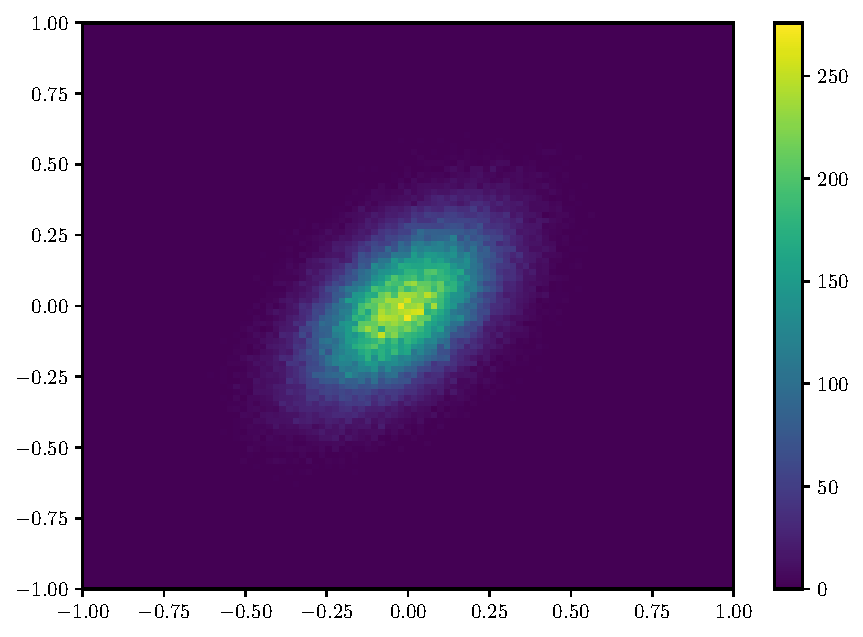
\includegraphics[width=0.25\textwidth]{plots/3Dgaussian_posdef/3-1_FAKE_100000_100_3_5_2_10000_128_0.5.pdf}
  \caption{\label{fig:3dgauss}Example of samples generated for a 3D correlated
  multivariate normal distribution using a QGAN generator model.}
\end{figure*}

\section{Generating LHC events}
\label{sec:lhc}

\begin{enumerate}
  \item Show ttbar and WW results, histograms, KL, correlations, etc.
  \item Provide hints concerning data augmentation.
  \item Show experimental results obtained with quantum hardware, identify the
  best features, pro and cons of different hardware.
\end{enumerate}

\begin{figure*}
  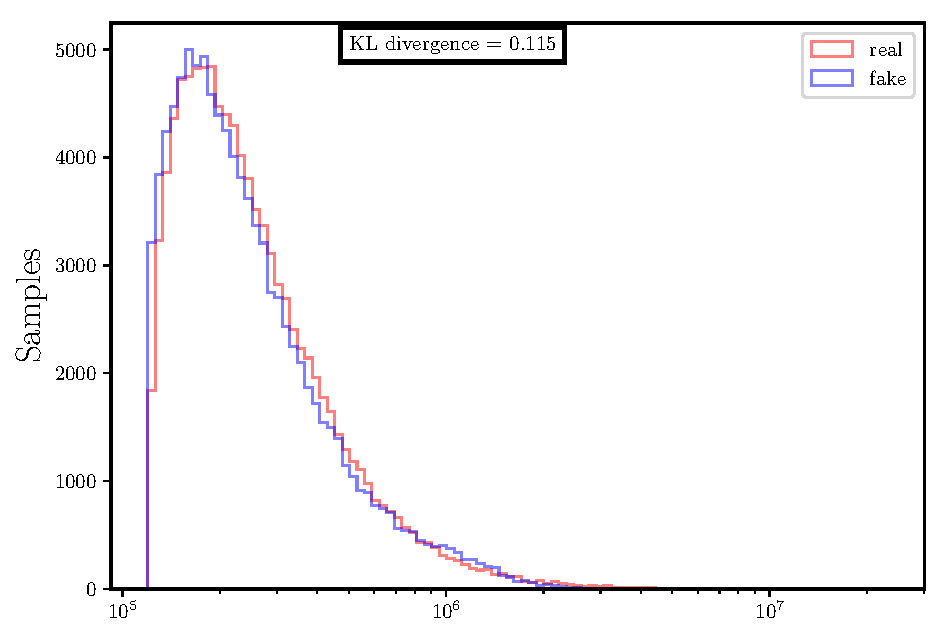
\includegraphics[width=0.25\textwidth]{plots/LHCttbar/s-distribution_100000_100_3_5_4_10000_128_0.5.pdf}%
  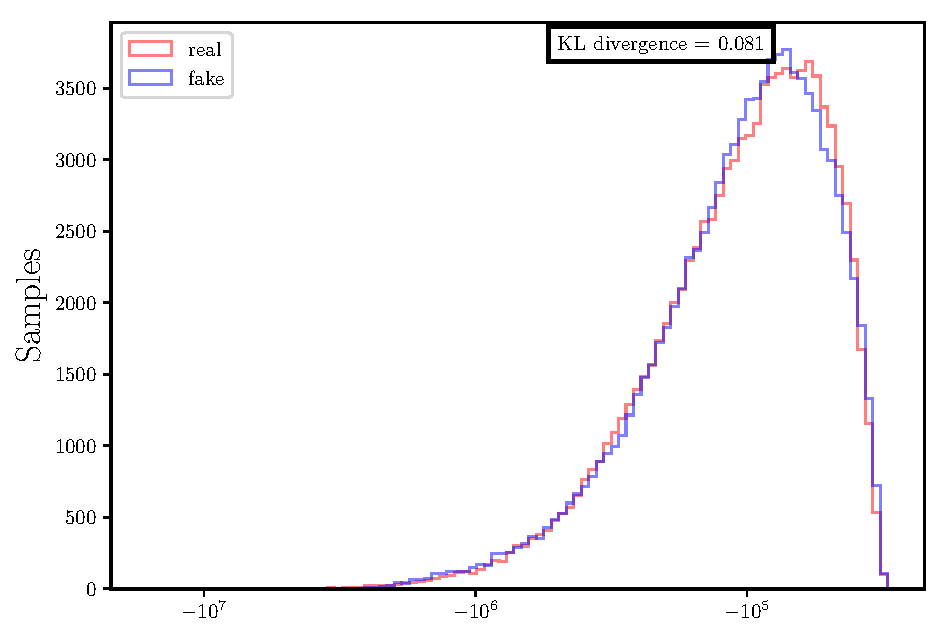
\includegraphics[width=0.25\textwidth]{plots/LHCttbar/t-distribution_100000_100_3_5_4_10000_128_0.5.pdf}%
  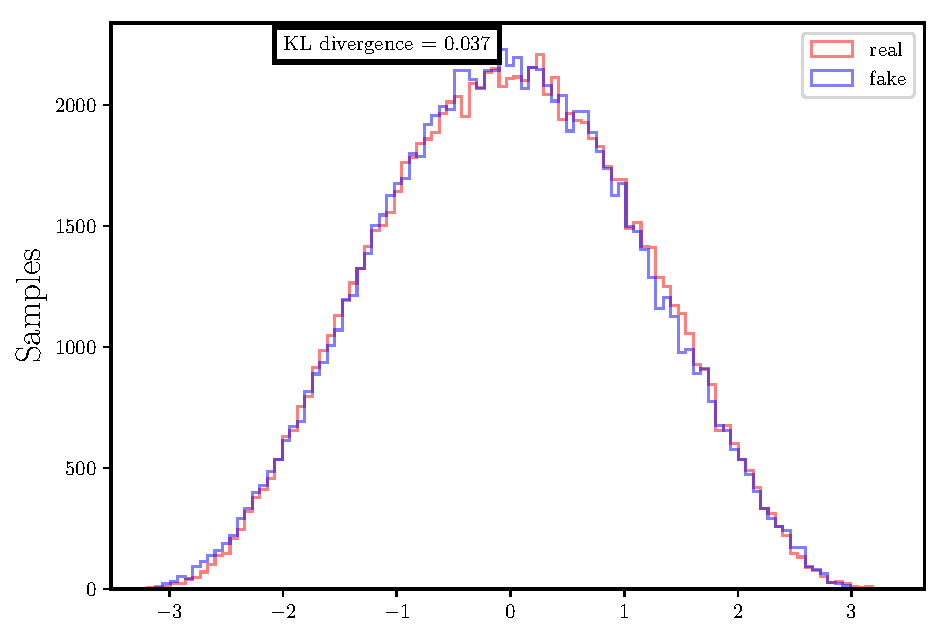
\includegraphics[width=0.25\textwidth]{plots/LHCttbar/y-distribution_100000_100_3_5_4_10000_128_0.5.pdf}

  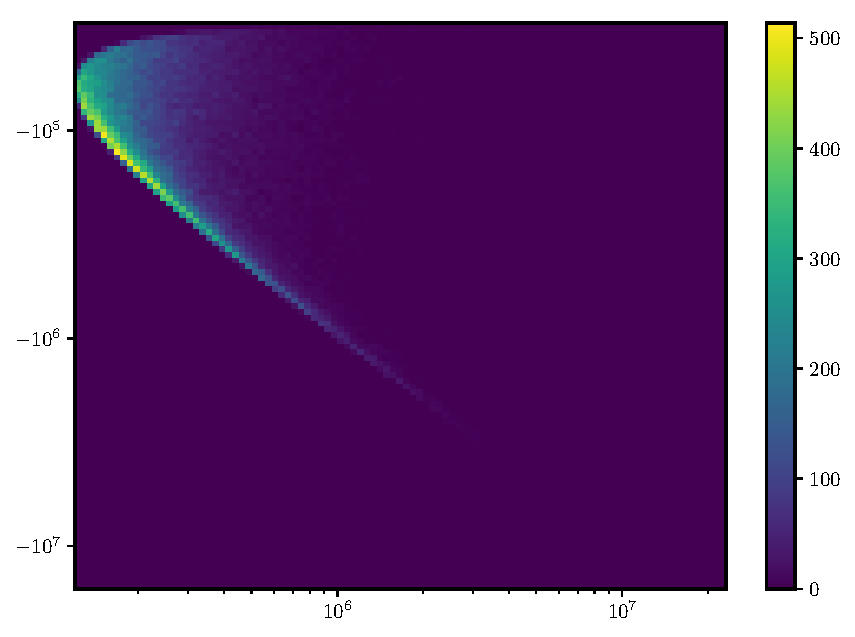
\includegraphics[width=0.25\textwidth]{plots/LHCttbar/s-t_REAL_100000_100.pdf}%
  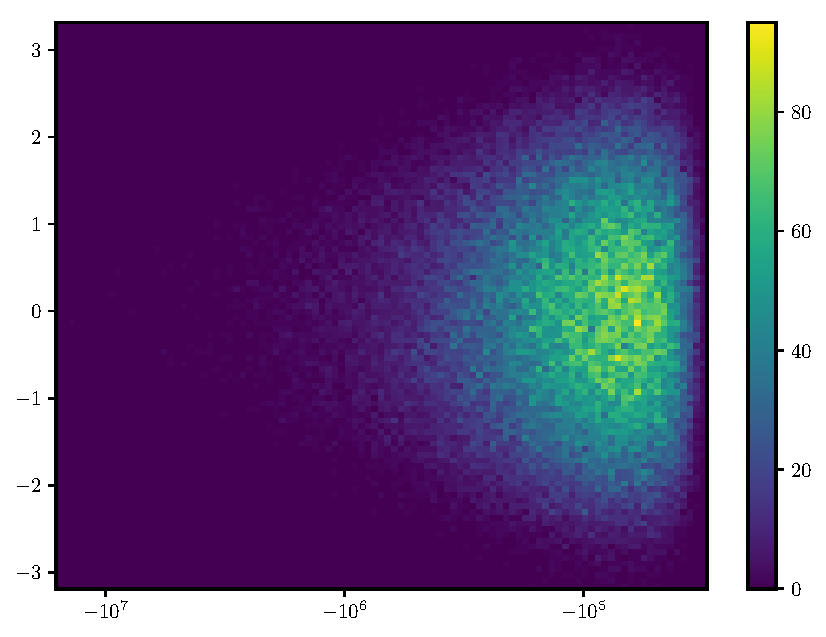
\includegraphics[width=0.25\textwidth]{plots/LHCttbar/t-y_REAL_100000_100.pdf}%
  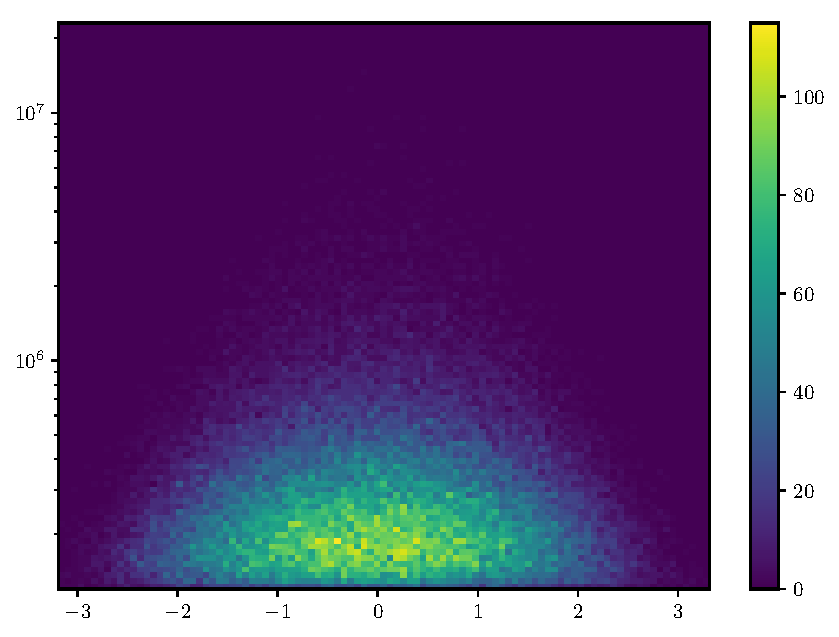
\includegraphics[width=0.25\textwidth]{plots/LHCttbar/y-s_REAL_100000_100.pdf}

  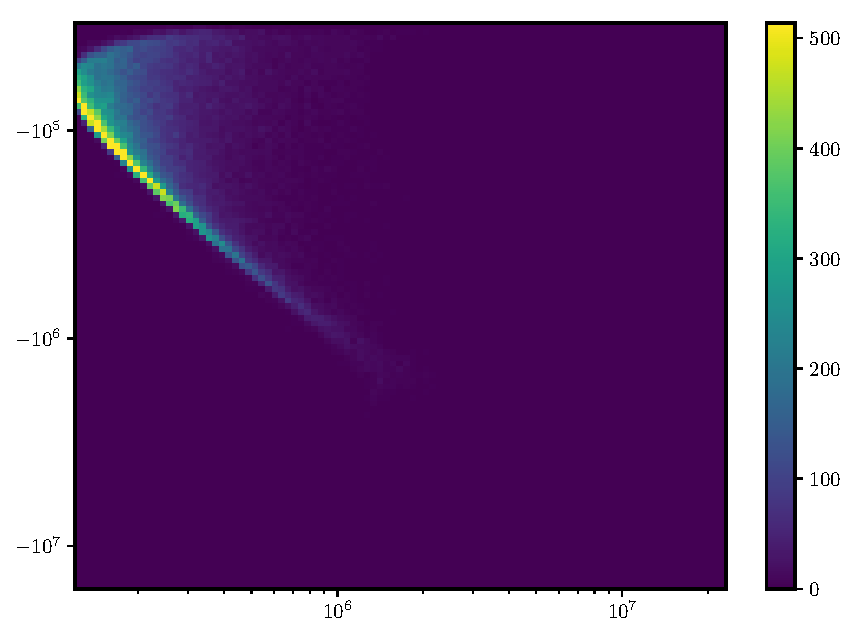
\includegraphics[width=0.25\textwidth]{plots/LHCttbar/s-t_FAKE_100000_100_3_5_4_10000_128_0.5.pdf}%
  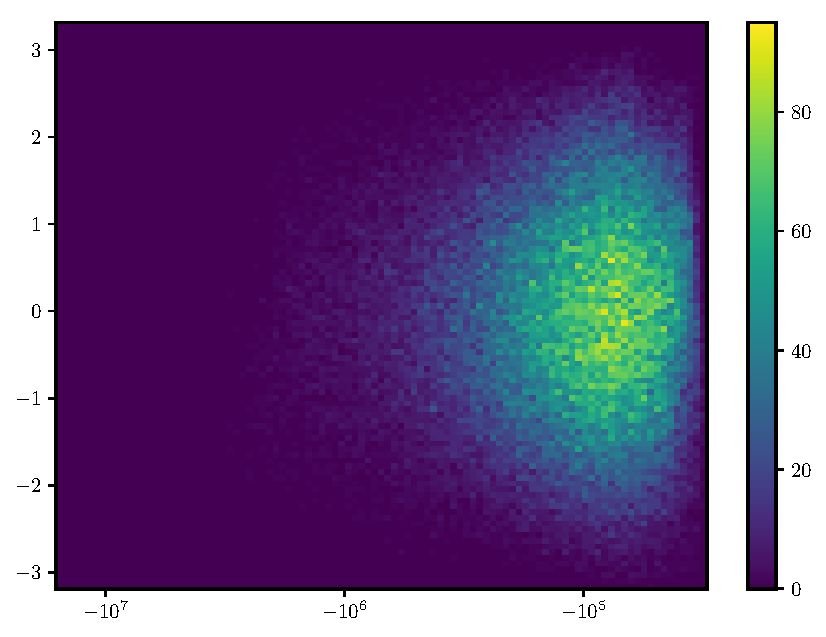
\includegraphics[width=0.25\textwidth]{plots/LHCttbar/t-y_FAKE_100000_100_3_5_4_10000_128_0.5.pdf}%
  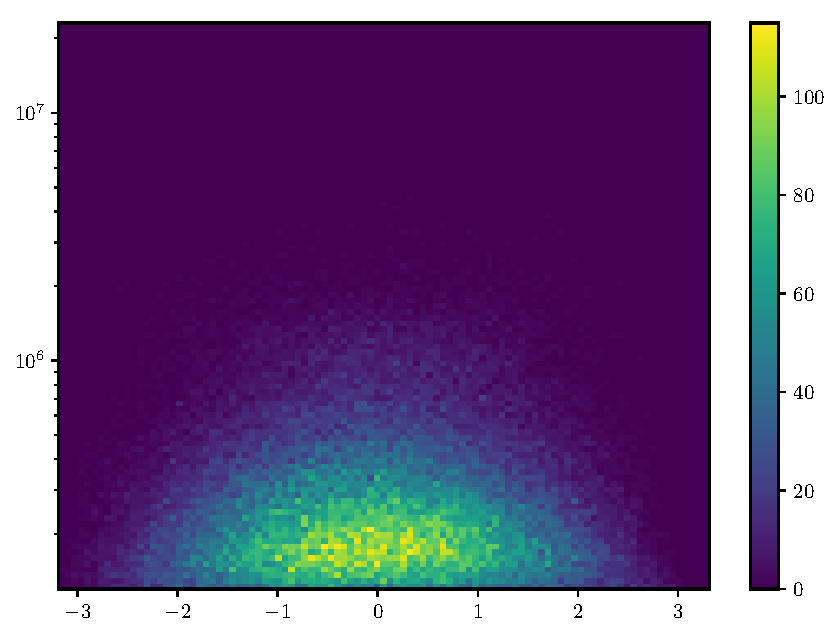
\includegraphics[width=0.25\textwidth]{plots/LHCttbar/y-s_FAKE_100000_100_3_5_4_10000_128_0.5.pdf}

  \caption{\label{fig:3dgauss}Example of samples generated for a $t\bar{t}$
  production using a QGAN generator model.}
\end{figure*}

\section{Sampling from real quantum hardware}
\label{sec:deployment}

{\color{red}[SC: Julien and Marco please summarize the experimental setup]}

\begin{figure*}
  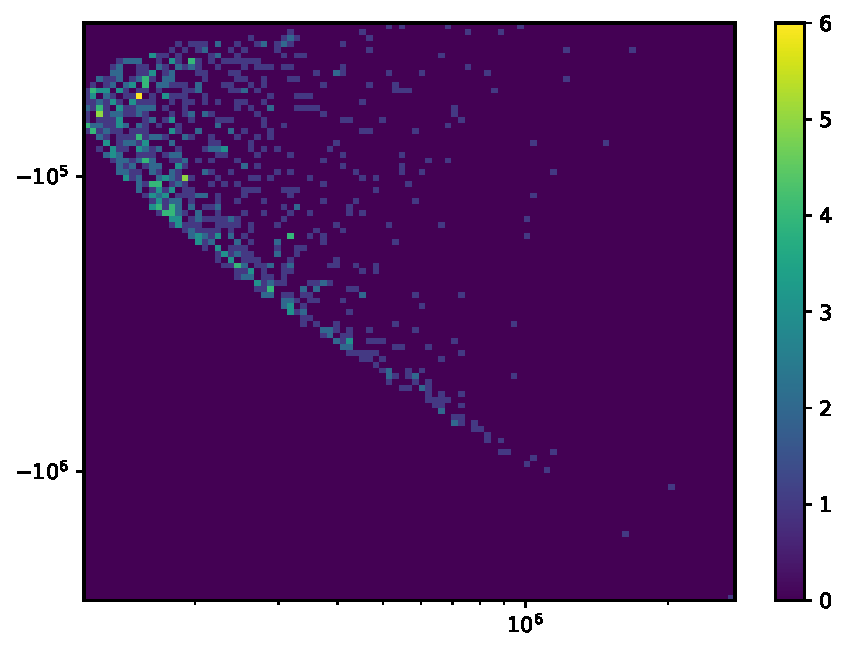
\includegraphics[width=0.25\textwidth]{plots/hardware_1k/ibm_lagos/s-t_REAL_1000_100.pdf}%
  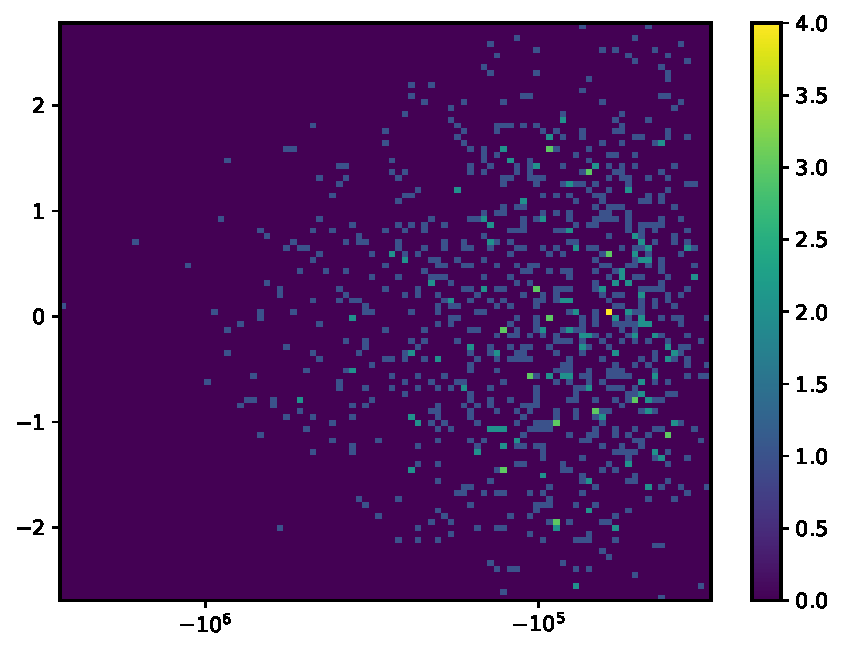
\includegraphics[width=0.25\textwidth]{plots/hardware_1k/ibm_lagos/t-y_REAL_1000_100.pdf}%
  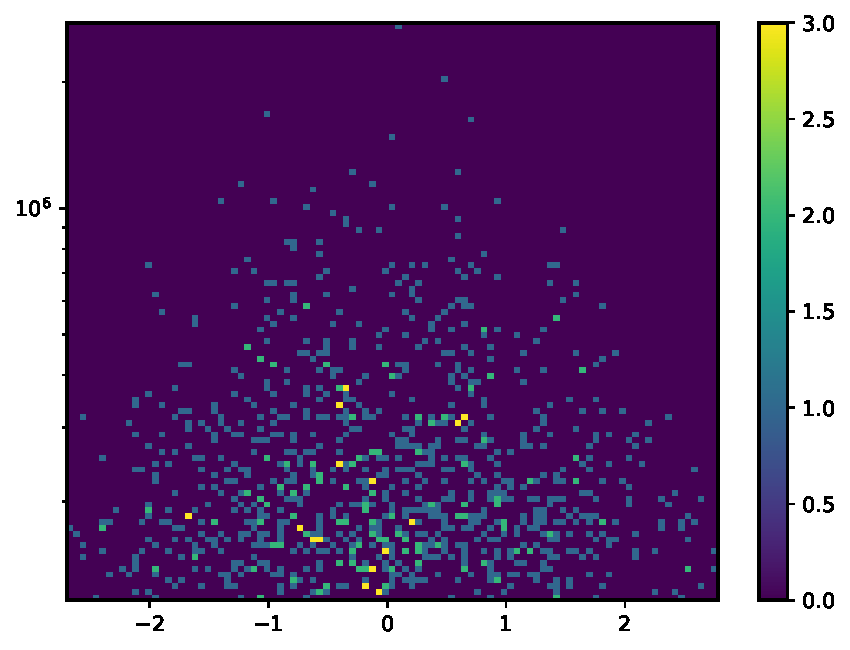
\includegraphics[width=0.25\textwidth]{plots/hardware_1k/ibm_lagos/y-s_REAL_1000_100.pdf}

  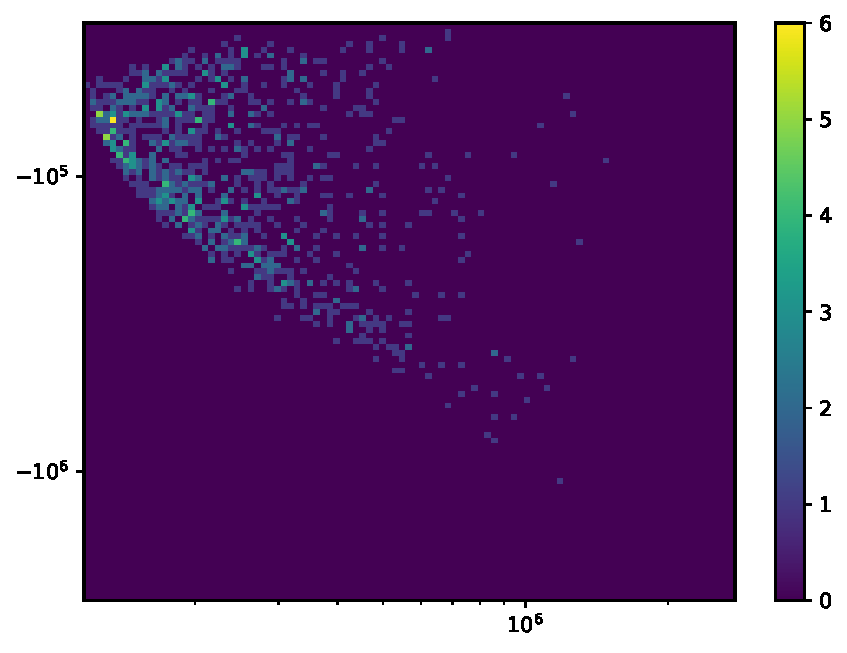
\includegraphics[width=0.25\textwidth]{plots/hardware_1k/ibm_lagos/s-t_FAKE_1000_100_3_5_2_10000_128_0.5_1024.pdf}%
  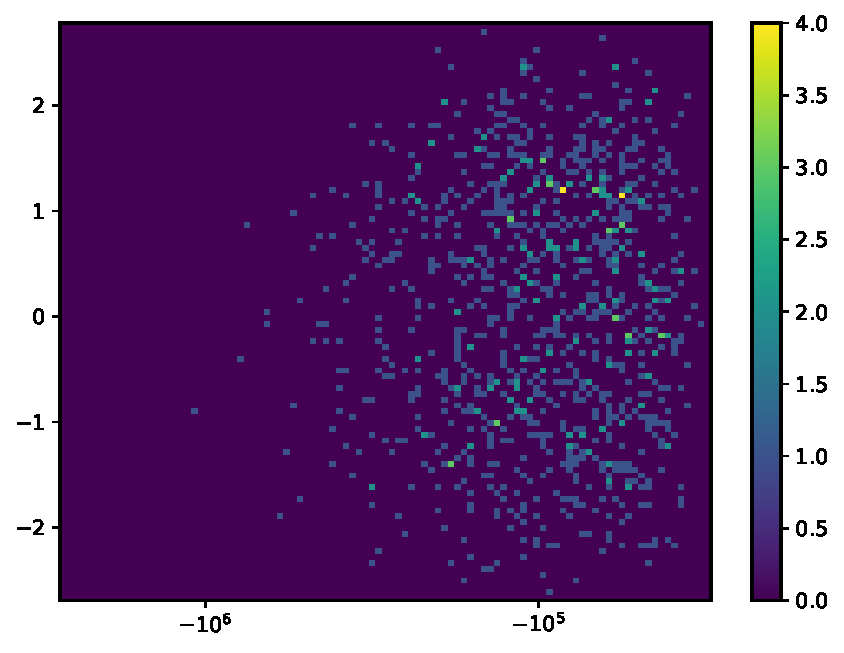
\includegraphics[width=0.25\textwidth]{plots/hardware_1k/ibm_lagos/t-y_FAKE_1000_100_3_5_2_10000_128_0.5_1024.pdf}%
  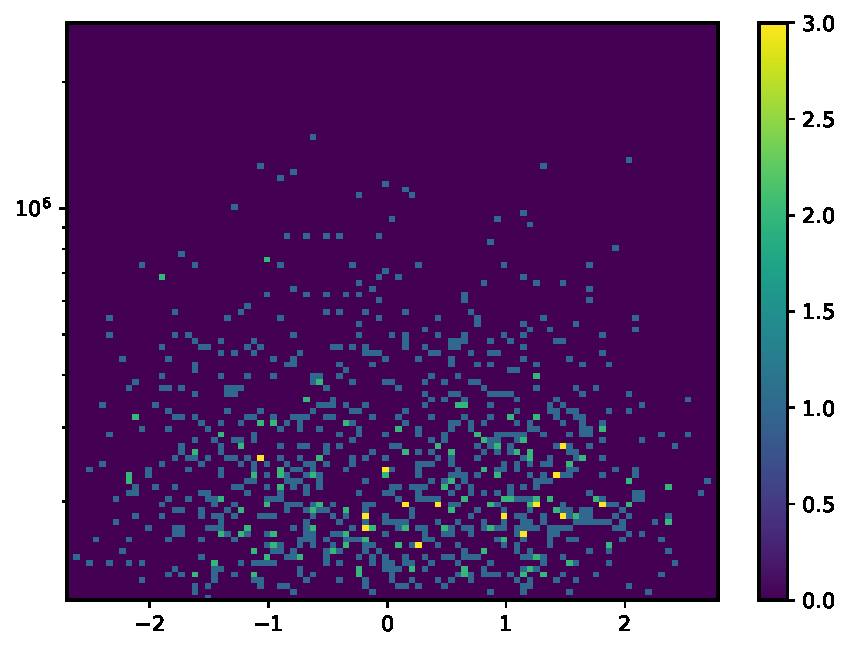
\includegraphics[width=0.25\textwidth]{plots/hardware_1k/ibm_lagos/y-s_FAKE_1000_100_3_5_2_10000_128_0.5_1024.pdf}

  \caption{\label{fig:3dgauss}Example of samples generated for a $t\bar{t}$
  production using a QGAN generator model on IBM Lagos.}
\end{figure*}

\begin{figure*}
  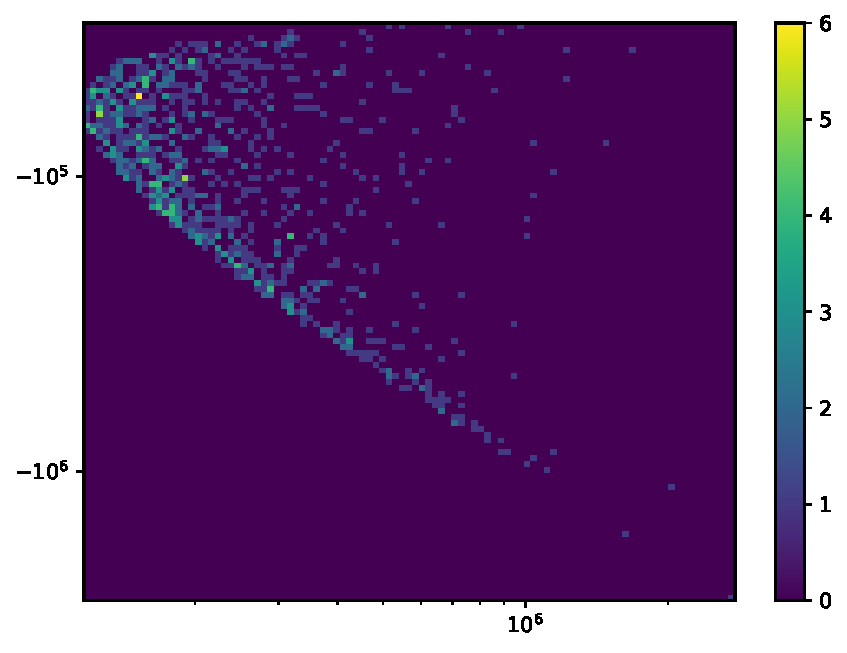
\includegraphics[width=0.25\textwidth]{plots/hardware_1k/ionQ/s-t_REAL_1000_100.pdf}%
  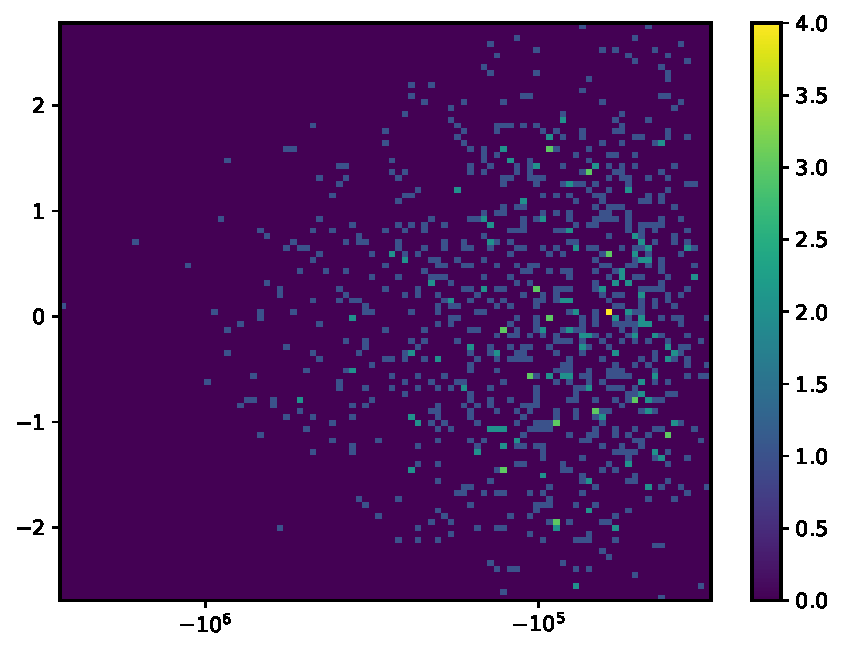
\includegraphics[width=0.25\textwidth]{plots/hardware_1k/ionQ/t-y_REAL_1000_100.pdf}%
  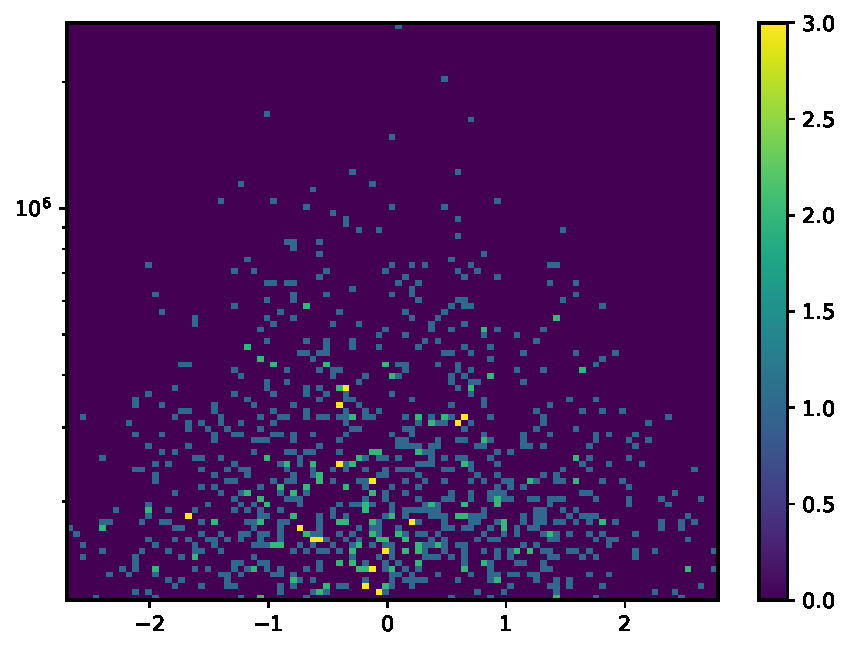
\includegraphics[width=0.25\textwidth]{plots/hardware_1k/ionQ/y-s_REAL_1000_100.pdf}

  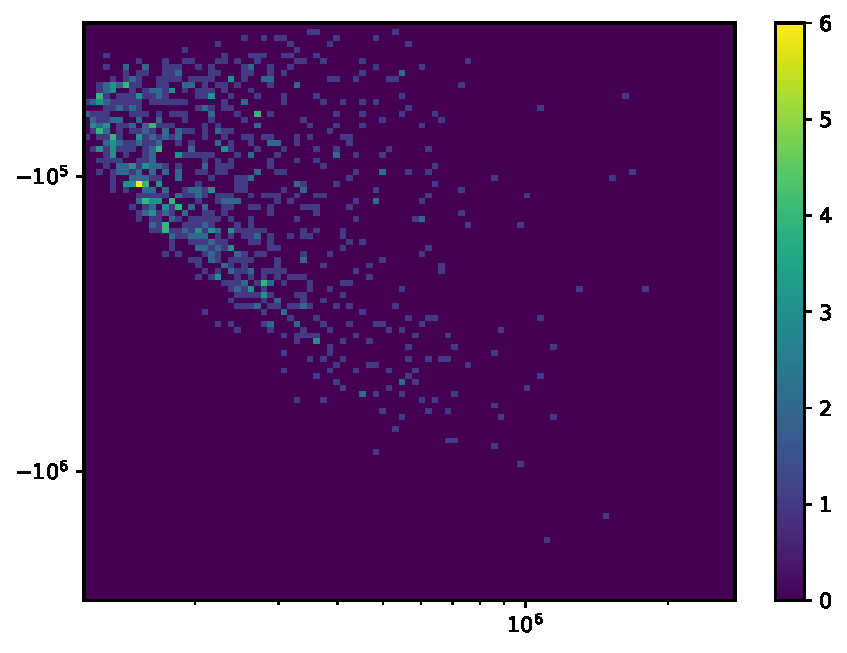
\includegraphics[width=0.25\textwidth]{plots/hardware_1k/ionQ/s-t_FAKE_1000_100_3_5_2_10000_128_0.5_1024.pdf}%
  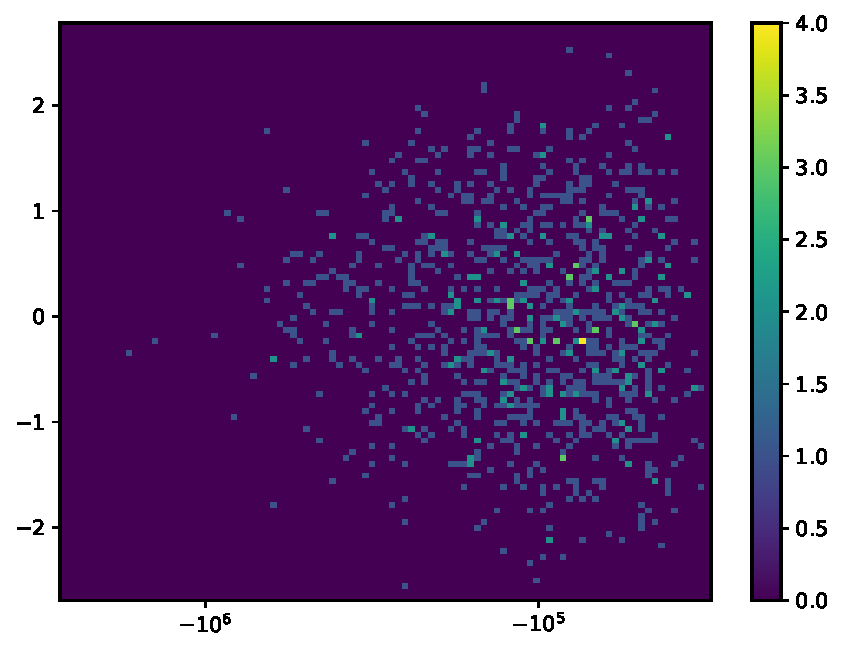
\includegraphics[width=0.25\textwidth]{plots/hardware_1k/ionQ/t-y_FAKE_1000_100_3_5_2_10000_128_0.5_1024.pdf}%
  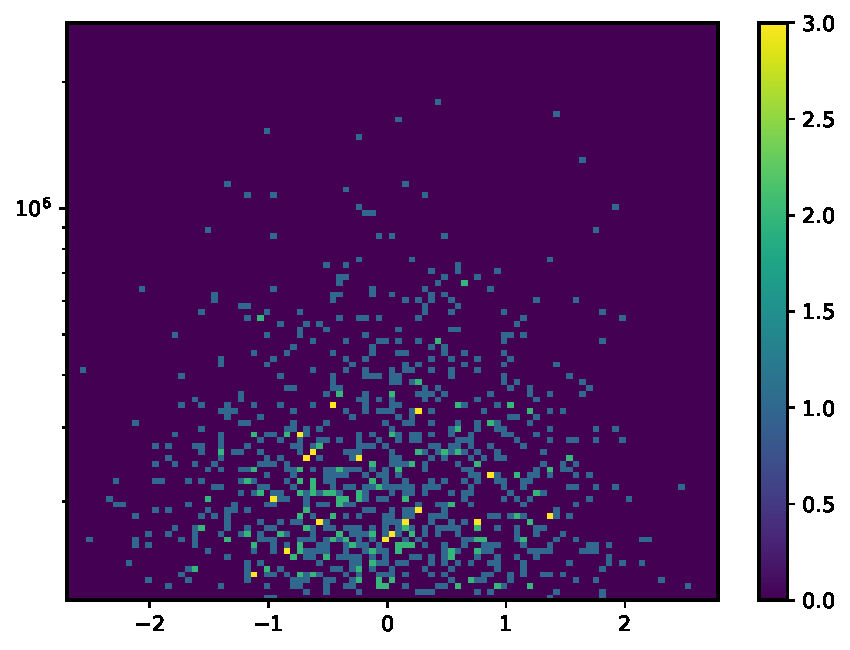
\includegraphics[width=0.25\textwidth]{plots/hardware_1k/ionQ/y-s_FAKE_1000_100_3_5_2_10000_128_0.5_1024.pdf}

  \caption{\label{fig:3dgauss}Example of samples generated for a $t\bar{t}$
  production using a QGAN generator model on IonQ.}
\end{figure*}


\section{Correlation analysis}

{\color{red}[SC: Anthony please summarize your results]}

\section{Conclusion}
\label{sec:conclusion}

In this work we proposed variational quantum circuit models for the generation
of Monte Carlo events in the context of high energy physics (HEP). We have
investigated and identified the most suitable Ansatz for the parametrization of
a quantum generative network. Using quantum circuit simulation on classical
hardware, we show that {\tt QGMC} generators are suitable for Monte Carlo event
simulation.

We highlight some advantages of the {\tt QGMC} model when compared to the standard
machine learning methodology. From a hardware implementation point of view, the
possibility to write the specific {\tt QGMC} circuit in a quantum processor, using
its primitives (gates), will accelerate the evaluations and training performance
of Monte Carlo sampling. We expect that real quantum devices will be more
efficient in terms of energy power than classical hardware based on hardware
accelerators such as graphical process units (GPUs).

Furthermore, we propose a reconstruction method for evaluating the {\tt QGMC}
model in a real quantum device using measurements. This procedure brings all the
difficulties that are typical of experimental quantum hardware, including noise,
error corrections and decoherence. The implementation of accurate and stable
{\tt QGMC} in a real quantum device still requires the development of hardware
architecture with lower gate error tolerances in comparison to the current
available machines.

On the other hand, our results should be considered as a proof-of-concept
exercise, given that the quantum simulation performance are still not
competitive with an equivalent machine learning implementation. The {\tt QGMC}
approach may show advantages when more precise quantum devices will be
available.

Nevertheless, this is a first attempt to bridge the power of quantum machine
learning algorithms into the complexity of Monte Carlo simulation in HEP. We
wish that the approach presented here will inspire new HEP applications which
may benefit from quantum computing.

{\color{red}{C: Include references HEP somewhere in the conclusions:  there also exist some examples of quantum algorithms designed to
address some problems in high energy physics
(HEP)~\cite{Perez-Salinas:2020nem,hep_amplitudes-bepari2020, hep_simulation-bauer2019,
hep_gluon-alexandru2019, hep_parton-lamm2020}.}}

\acknowledgments

This project is supported by CERN's QTI. SC is supported by the European
Research Council under the European Union's Horizon 2020 research and innovation
Programme (grant agreement number 740006).

\bibliography{qgan.bib}

\end{document}
